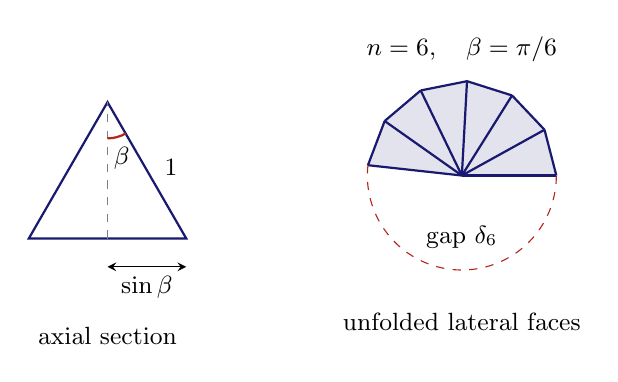
\begin{tikzpicture}[x=1cm,y=1cm,font=\small,>=stealth]
\begin{scope}[x=2cm,y=2cm]
\draw[MidnightBlue,thick] (-.5,0)--(0,.8660254)--(.5,0)--cycle;
\draw[gray,dashed] (0,0)--(0,.8660254);
\draw[BrickRed,thick] (0,.6360254) arc[start angle=-90,end angle=-60,radius=.23];
\node at (.09,.51) {$\beta$};
\node[right] at (.3,.45) {$1$};
\draw[<->] (0,-.18)--node[below] {$\sin\beta$}(.5,-.18);
\node[below] at (0,-.5) {axial section};
\end{scope}
\begin{scope}[shift={(4.5,.8)},scale=1.2]
\def\ang{28.95502437}
\fill[MidnightBlue!12] (0,0)--(0:1)--(\ang:1)--({2*\ang}:1)--({3*\ang}:1)--({4*\ang}:1)--({5*\ang}:1)--({6*\ang}:1)--cycle;
\foreach \k in {0,...,6} {\draw[MidnightBlue,thick] (0,0)--({\k*\ang}:1);}
\foreach \k in {0,...,5} {\draw[MidnightBlue,thick] ({\k*\ang}:1)--({(\k+1)*\ang}:1);}
\draw[BrickRed,dashed] ({6*\ang}:1) arc[start angle={6*\ang},end angle=360,radius=1];
\node at (270:.65) {gap $\delta_6$};
\node[above] at (0,1.1) {$n=6,\quad\beta=\pi/6$};
\node[below] at (0,-1.35) {unfolded lateral faces};
\end{scope}
\end{tikzpicture}
